%# -*- coding:utf-8 -*-
\documentclass[12pt,a4paper]{article}
\usepackage{buaa_paper}
\usepackage{hyperref}
\usepackage{fix-cm}
\usepackage{amsmath}
\title{Intership Report for the Degree of Master}
\schoolname{Sino-French Engineer School}
\papertitle{Research and Produce of Conversation Generation Models}
\researcharea{NLP Intern}
\studentnumber{ZY1624134}
\advisorin{XXX}
\advisorout{XXX}
\author{Shi Libin}
\date{Oct.15, 2018}

\begin{document}

\maketitle
\newpage
\tableofcontents
\newpage
%\newpage

\section{Basic Information}

\subsection{Internship}
\begin{itemize}
  \item Company: Microsoft STC Asia
  \item Company Logo: 
  \begin{figure}[!h]
    \centering
    
\includegraphics[width=0.5 \linewidth]{figures/logo.png}
  \end{figure}
  \item Company Address: \#5 Danling Street, Haidian District, Beijing, China
  \item Department: XIAOICE
  \item Internship Position: NLP Intern
  \item Internship Tutor: xxx
  \item Tutor's E-mail: \href{xxx@xxx.com}{xxx@xxx.com}
  \item Internship Dates: 
  \item School Advisor: xxx
  \item Adivsor's E-mail: \href{xxx@xxx.com}{xxx@xxx.com}
  \item Student: Shi Libin (Olivier)
  \item Student's E-mail: \href{olivier.shi@buaa.edu.cn}{olivier.shi@buaa.edu.cn}
  \item Option: ITR
\end{itemize}

\subsection{Introduction}

From the beginning of postgraduate entrance, I conducted research on the direction of Natural Language Processing (NLP) under the guidance of the computer college teacher Rong Wenge. And in that moment, i has set a goal to go to Microsoft to study. So in more than a year, I have been concentrating on the basic knowledge in the direction of NLP, and I have actively studied the cutting-edge and advanced technology of the academic field in the related fields. I finally entered Microsoft XIAOICE team for a six-month internship in May 2018.

Microsoft XIAOICE belongs to Microsoft STC Asia. Since its launch in China on May 30, 2014, it has been a technology-leading position in the field of chatbots driven by Artificial Intelligence (AI). During the internship in the Microsoft XIAOICE Chatbot Group, I am in charge of the research of the intelligent conversation algorithms, the reproduce and experimental comparison of the frontier models and the optimization, and finally to put the optimized model in online production. In the process, first of all, I realize that the knowledge I need to use is the natural language processing (NLP) and deep learning (DL) algorithms. In addition, the computer programming languages used in the work process are Python and C\#, and I use the Google's open source TensorFlow framework as my deep learning framework language since the work includes research and produce of deep learning algorithms.

Secondly, after mastering these basic knowledge, I read a lot of frontier academic papers on conversation generation models and retrieval models used in intelligent chatbots, and implement the methods in these frontier papers in the same time. Then I apply these frontier methods in our chatbots, and the model training and optimization have been carried out on the actual conversation data of XIAOICE. And a large number of experimental studies have been done on these models. 

Finally, in the process of learning and experiments, I summarize and analyze the advantages and disadvantages of different models, and then put the best model into the online codes and go to productuin, which is used in the daily chat application of the actual XIAOICE chatbot.


In this process, my main work can be divided into the following two aspects:
\begin{itemize}
  \item Optimization of the single-round conversation generation model. I use the Sequence-to-Sequence as the basic model framework, and then i design and improve the model based on the observation of the data and problem analysis of different models. Through a large number of contrast experiments, it can be proved that my model can improve the quality of conversation generation. Then i formalize the codes into online C\# codes, and use it to serve the online chat application in XIAOICE chatbot.

  \item Multi-round conversation generation model with context information. I first extract keywords from the historical information of multi-round conversation, including nouns, verbs, and adjectives, and regard them as keywords. Then i input these keywords into the neural networks to generate vectorized representation, and fuse these vectorized keywords with the user's query information, then use them to generate the response. This method can add historical multi-round conversation information in the ordinary Sequence-to-Sequence framework, and when the XIAOICE chatbot is used for multi-round conversation, it can keep logically consistent, and the dialogue is more natural and smooth.

\end{itemize}

\section{Single-round conversation generation model}
\subsection{Background}

For the single-round conversation task, it was handled based on the retrieval model before the Sequence-to-Sequence model framework was proposed~\cite{DBLP:conf/sigir/YanSW16}. Briefly introduce this method: 1) The first step is to crawl the data of people's daily chats from some social networks, prepare and clean out a large number of query-response pairs, and then store them in the database to build the index. 2) The second step, in the actual application, when the user inputs a sentence, and then uses the sentence as the query to retrieve the closest queries in the database, and returns the responses corresponding to these queries as candidates. 3) In the third step, the well-trained ranking model is used to sort the relevance of query and the candidate responses, and then the most relevant candidate is returned to the user. In these processes, the second step is equivalent to roughly select a part of the candidate set from the large amount of data in the database, and the third step is equivalent to selecting the most appropriate reply.

Some of the problems can be seen from the general workflow of this retrieval-based conversation methods. For example, it needs huge numbers of data to build the database, it requires high quality for the prepared query-response pairs. In addition, when the response obtained by this method is returned as a reply to users, users will soon find that the data is crawled from the social networks, which makes the robot lack flexibility and intelligence.

As a result, an automatic dialogue method based on the generation model has emerged, and this conversation generation model has been a hot topic in academic circles and industry in recent years. Among the various conversation generation models, the best match for the conversation scene is Sequence-to-Sequence (seq2seq) framwork~\cite{DBLP:journals/corr/VinyalsL15,DBLP:journals/corr/WuSCLNMKCGMKSJL16}. As the name suggests, the first sequence is the query sentence entered by the user, and the second sequence is the response sentence which is condisioned on the query sentence. The overview of this framework can be easily formalized in a mathematical form: given a query sentence which is a sequence of words input, ${X=\{x_1, x_2, ..., x_n\}}$, the goal of our model is to generate a reply which is a sequence of words output, ${Y=\{y_1, y_2, ..., y_m\}}$. So, the work for building the model that needs to be done is to calculate a conditional probability:
\begin{gather*}
  P(Y|X) = P(y_1, y_2, ..., y_m|x_1, x_2, ..., x_n)
\end{gather*}

The complete structure of the model we built is shown in Fig.~\ref{fig:arch}. Next I will give a brief introduction to each module of this model.
\begin{figure}[!ht]
  \centering
  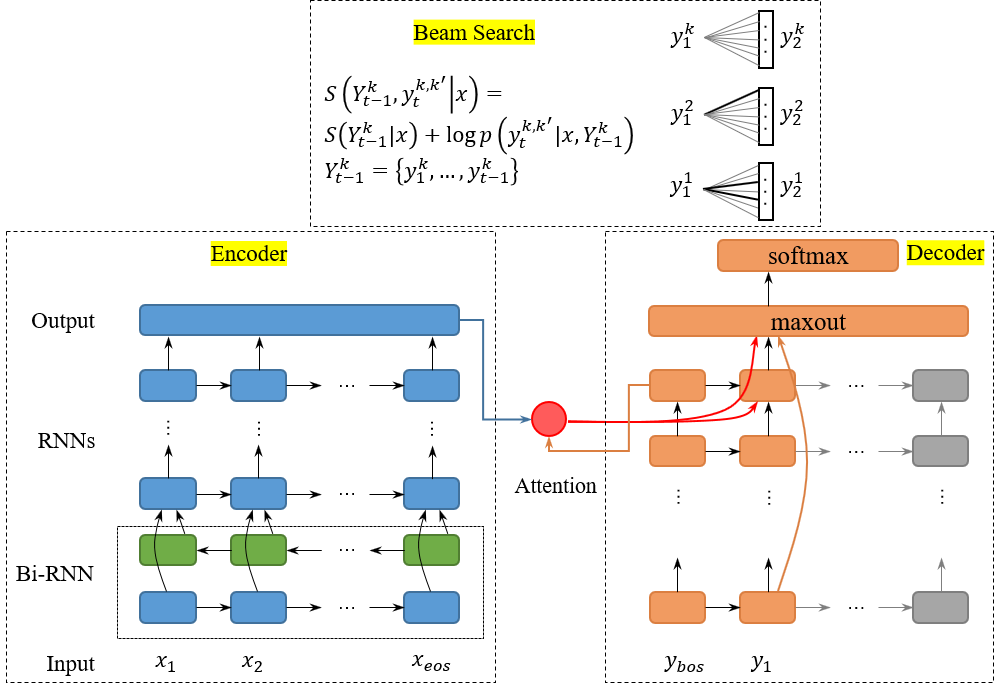
\includegraphics[width=0.96\linewidth]{./figures/seq2seq_beamsearch.png}
  \caption{seq2seq framework}\label{fig:arch}
\end{figure}


\subsection{seq2seq}

\noindent{\textbf{Encoder:}}
\begin{itemize}
  \item input layer: query sequence
  \item RNNs layers: the first layer is bidirectional RNNs (Bi-RNNs), and the second layer as well as the above layers are stacked multi-layer unidirectional RNNs
  \item output layer: the output is the encoded information for the query sequence, which is the complete context for the decoder.
\end{itemize}

\noindent{\textbf{Decoder:}}
\begin{itemize}
  \item input layer: response sequence, it requires distinguishing the training and inference phases: in the training phase, it is the way of teacher forcing learning (each step inputs are ground truth words); while in the inference phase, each step inputs are the last generative outputs.
  \item RNNs layers: the first layer to the penultimate layer are standard multi-layer unidirectional RNNs, and the last layer is the RNN layer with attention.
  \item output/predict layer: first use maxout to do a fusion of the RNN outputs, the attentioned context, and the embedded inputs, and then use softmax to predict.
\end{itemize}


\subsection{Attention mechanism}
The encoder outputs contains the entire context information, but when the model generates at each step, it may focus on diffent words in the context information. So we should add the attention mechanism to the model that weights the context words at each generation step. This is called alignment model in neural machine translation (NMT) because there is a strong correspondence between words in different languages. 

Literature tells us that there are two types of attention mechanism, called Bahdanau attention~\cite{DBLP:journals/corr/BahdanauCB14} and Luong attention~\cite{DBLP:conf/emnlp/LuongPM15}. In my work, I have explored them both, and their formulas are as follows:

\noindent{\textbf{Bahdanau attention:}}
\begin{figure}[!htbp]
  \centering
  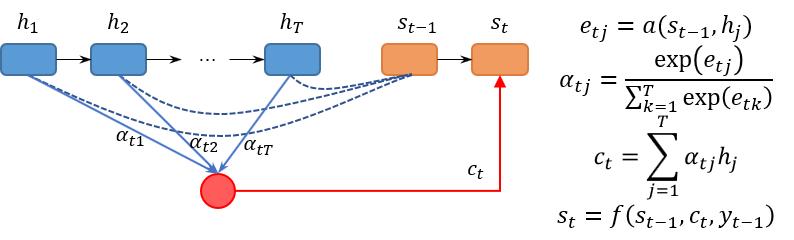
\includegraphics[width=0.8\linewidth]{./figures/attention_bahdanau.png}
  \caption{bahdanau attention}\label{fig:bahdabau}
\end{figure}

\noindent{\textbf{Luong attention:}}
\begin{figure}[!htbp]
  \centering
  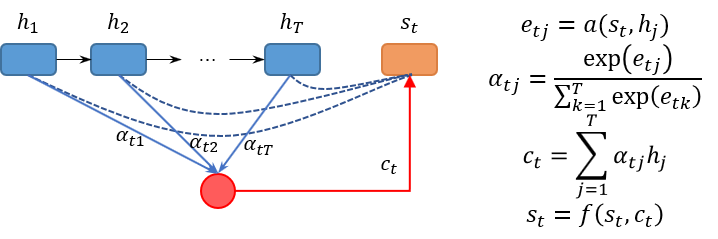
\includegraphics[width=0.8\linewidth]{./figures/attention_luong.png}
  \caption{luong attention}\label{fig:luong}
\end{figure}


\subsection{Maxout}
Maxout technique is said as to highlight some of the valid feature signals~\cite{DBLP:conf/icml/GoodfellowWMCB13}, and it is a basic but important technique for NLP task. Specifically in my implementation, it first fuse the RNN outputs $s_{t-1}$, attentioned context $c_t$, and embedded inputs $Ey_{t-1}$,and then reduce the dimension with max pooling. If we set the dimension that reduces to as $l$, then we have,
\begin{gather*}
  \tilde{v}_t =U_0 s_{t-1} + W_0 Ey_{t-1} + C_0 c_t \\
  v_t = [\mathrm{max}\{\tilde{v}_{t,2j-1}, \tilde{v}_{t,2j}\}]_{j=1,...,l} \\
  p(y_t|s_{t-1}, y_{t-1}, c_t) = \mathrm{softmax}(v_t)
\end{gather*}


\subsection{Loss function}
The loss function uses the cross entropy function~\cite{DBLP:conf/iccv/LinGGHD17}, that is, when generating a word at each step, the generated task is regarded as a multi-class problem. It means we take each word in the vocabulary as a class, and we need select the most suitable word in the vocabulary.

\noindent{\textbf{Cross entropy:}}
\begin{equation*}
  \mathrm{CE}(\tilde{y}, y) = - \sum_{t}{y_t \mathrm{log}\tilde{y}_t}
\end{equation*}


\subsection{Beam search}
\begin{figure}[!htbp]
  \centering
  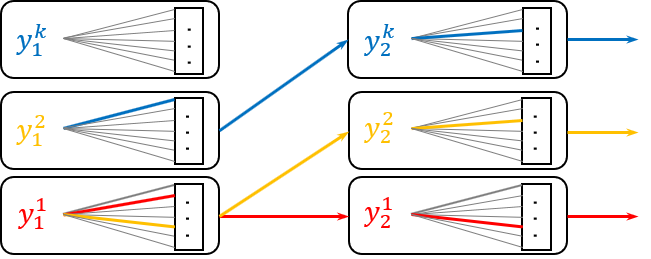
\includegraphics[width=0.9\linewidth]{./figures/beam_search.png}
  \caption{beam search}\label{fig:beam_search}
\end{figure}
\begin{gather*}
    S(Y_t|x) = S(Y_{t-1},y_t|x) = \max \mathrm{sort}_{K}{S(Y_{t-1}^k,y_t^{k,k'}|x)_{k,k' \in K}} \\
    S(Y_{t-1}^k,y_t^{k,k'}|x) = S(Y_{t-1}^k|x) + s_t^{k,k'} \\
    s_t^{k,k'} = \log p(y_t^{k,k'}|x, Y_{t-1}^k) \\
    Y_{t-1}^k = \{y_1^k, \cdots, y_{t-1}^k\}
\end{gather*}

In the formula, $S(Y_t^k)$ denotes the probability of the sequence $Y_t^k$, and is calculated by $\log(\mathrm{softmax})$. $y_t^{k,k'}$ denotes the $t$ step of generation, and the $k$-th beam branch, and the $k'$-th word, and then $s_t^{k,k'}$ denotes the probability of generationg this word. $K$ denotes the width of beam search, which is a hyper-parameter. $\max \mathrm{sort}_{K}$ stands for selecting the highest $K$ words by descending order.


For this formula, i design the tricks from two aspects to adjust the beam search:
\begin{itemize}
  \item Adjustment for prefix of the generating sequence, that is to adjust $S(Y_t^k)$.
  \item Adjustment for the current generative step, that is to adjust $s_t^k$.
\end{itemize}




\subsection{Discussion}
\subsubsection{parameter}
In order to make the model more capable of learning, in addition to adding a variety of mechanisms to the model to make the model more complex (as mentioned above), we can also increase the size of the parameters in the model.

\begin{itemize}
  \item RNN layer size:two-layer is better than one-layer. According to the experiment, The two-layer seq2seq network converges to $\mathrm{PPL} = 21$ in 5 iterations, while the one-layer seq2seq requires 9 iterations. So, two-layer seq2seq is better both from the convergence speed and the final generating performence. 
  \item parameter size:the parameter size here includes embedding size and hidden size. According to the experimental results, the larger the parameter amount, the better the model's performance.
\end{itemize}

\subsection{Experiments and Results}
In order to prove that the effect of our model can meet the requirements of online product application, we have done some experiments. The first is the experimental setup:
\begin{itemize}
  \item Dataset:we use two kinds of data, one is the chat data crawled from the social network, and the other is the internal chat data of XIAOICE. After cleaning, we prepare a dataset of 20 million number.
  \item Metrics:the metrics we use contain three types: 1) Perplexity (PPL) that uses to measure the language passability~\cite{DBLP:journals/coling/BrownPPLM92}. 2) Distinct that uses to measure the diversity of generation responses~\cite{DBLP:conf/naacl/LiGBGD16}. 3) Human evaluation, call human to annotate whether the generating response could reply the user query.
  \item Baselines:our main comparison model is the previous generation model of XIAOICE chatbot, which is based on the basic seq2seq model~\cite{DBLP:journals/corr/BahdanauCB14}.
\end{itemize}


The experimental results reflect that our new model has a certain improvement in the smoothness, relevance, and diversity of the generative responses, and fully meets the task requirements that the company has assigned to me. With this results, i transfer the Python codes into C\# codes as our online codes are written in C\#, and then put this model on the  product application of XIAOICE chatbot.

The work presented in this chapter is completed work, including researching methods, reproducing models, data preparation, experimental comparisons, and online works. The task to be introduced in the next chapter will be more difficult, so it is still in an experimental research stage.



\section{Multi-round conversation generation model with context information}

After completing the single-round conversation generation model, we conduct an in-depth analysis of the data of the XIAOICE chatbot and the user's actual dialogue scene, and soon find a serious problem. Although the results of the single-round generative conversation are very good, we can see that there are inconsistencies or even contradictories in the scene of multi-round conversations. For example,


\begin{quote}
> (1)用户: 今天天气真的好!(En: It is a nice day!) \\
> (2)小冰: 阳光明媚啊 (En: The sun is shining)\\
> (3)用户:希望明天也好好的 (En: Hop that tomorrow is also nice)\\
> (4)小冰:希望你也幸福 (en: Hop that you are also happy)
\end{quote}




\section{Conclusion}

The content of the internship at XIAOICE Group, Microsoft STC Asia, is mainly responsible for the investigation of the conversation generation model, including the construction and experiment of single-round and multi-round conversation models. Before I entered the company to take over this task, I did not touch the model and method related to this task. So, under the guidance of the company tutor, I read the relevant papers and supplemented the necessary knowledge in a short time, and then quickly started this task. And I finally complete this task excellently. And this internship experience and results have also enabled me to successfully obtain Microsoft's return offer, and lay a solid foundation for future work.

In this internship, I learned a lot of knowledge and skills, including deep learning, natural language processing, data processing mining and analysis, also including TensorFlow, Python, C$\#$, Git and other code skills. Moreover, after half a year of research and exploration on the model framework of Sequence-to-Sequence, I have a deep understanding and mastery of the model, which also formed my outstanding skills and competitiveness. In addition, in this internship life, I also made a wide range of friends, in the relaxed and comfortable working environment of Microsoft, we work hard and helped together.

\section{Acknowledgement}
Finally, I would like to thank my tutor at Microsoft XIAOICE. Although he is only 3 years older than me, he is already a very experienced researcher in deep learning and natural language processing. He gives me a lot of help, not only in terms of guidance of technical methods but also in terms of advising of how to study and learn. Secondly, I would like to thank Associate Professor Rong Wenge, a tutor at Beihang University, for his introduction of natural language processing and computer science. Finally, I would also like to thank the Sino-French Engineer School for a six-year course and training. Although many courses at school are not related to the current work, the experience of studying some courses in the high-pressure environment at school has greatly improved me, and the ability to self-learn and the ability to withstand stress is a valuable asset.


\newpage
%\addcontentsline{toc}{section}{参考文献}
\bibliography{bibs}

\end{document}
